\documentclass[11pt]{article}
\usepackage[usenames, dvipsnames]{color}
\usepackage[margin=1in,vmargin=1in]{geometry}
\usepackage[utf8]{inputenc}
\usepackage[english]{babel}
\usepackage{tikz}
\usepackage{pgfplots}
\usepackage{fancyhdr}
\pagestyle{fancy}
\usepackage{caption}
\usepgfplotslibrary{polar}
\usepgflibrary{shapes.geometric}
\usetikzlibrary{calc}
\pgfplotsset{compat=1.5.1}
\pgfmathdeclarefunction{gauss}{2}{%
  \pgfmathparse{1/(#2*sqrt(2*pi))*exp(-((x-#1)^2)/(2*#2^2))}%
}

\pgfmathdeclarefunction{bivar}{4}{%
  \pfgmathparse{1/(2*pi*#2*#4) * exp(-((x-#1)^2/#2^2 +
    (y-#3)^2/#4^2))/2}%
}
\usetikzlibrary{shadows}
%\usepackage{hyperref}
%\hypersetup{
%    colorlinks=true,
%    linkcolor=purduegold,
%    filecolor=magenta,      
%    urlcolor=cyan,
%}
%\urlstyle{same}
\usepackage{graphicx}
\usepackage{graphics}
\usepackage{amsmath}
\usepackage{amsthm}
\usepackage{amssymb}
\usepackage{float}
\DeclareMathOperator*{\argmin}{arg\,min}
\newcommand*{\everymodeprime}{\ensuremath{\prime}}
{\renewcommand{\arraystretch}{2}%
\usepackage [autostyle, english = american]{csquotes}
\usepackage[backend=bibtex]{biblatex}
\bibliography{Master}
\MakeOuterQuote{"}
\graphicspath{ {img/}}
\definecolor{purduegold}{cmyk}{.43,.56,1,0}
\newcommand{\mcolor}[2][red]{{\color{#1}\textbf{#2}}}

\usepackage{algorithm}
\usepackage[noend]{algpseudocode}
%\usepackage{fontspec}
%\setmainfont{Hoefler Text}
\newcommand*\DNA{\textsc{dna}}

\newcommand*\Let[2]{\State #1 $\gets$ #2}
%\algrenewcommand\alglinenumber[1]{
%    {\sf\footnotesize\addfontfeatures{Colour=888888,Numbers=Monospaced}#1}}
%\algrenewcommand\algorithmicrequire{\textbf{Precondition:}}
%\algrenewcommand\algorithmicensure{\textbf{Postcondition:}}
\title{Question: Iterative Learning/Backprop}
\author{}
\date{}
\begin{document}
\maketitle
\tableofcontents

Is is fair to assume that the error surface changes depending on the input? The error surface of a model is generally seen as something like the image below in figure \ref{fig:error_surface}. Since our goal is to find the ML solution of the weights given data, we need to see as much error as possible and find the correct weights. We do this doing using iterative updates in back propogation. And we say this is okay to do in a mini-batch setting, despite the fact that we arent using all the data, due to computational efficiency. However, technically each set of data would give a random error surface. All the error surfaces would come from the same distribution of error surfaces, given the model, but each mini-batch would be different. And when we iteravely update the error values, we don't know the "true" minimum... ever. So mini-batches are fine because a full-batch pass would only give a sample of the "true" minimum anyway. Therefore, for the sake of generalization and computational resources, we would use mini-batches.

How correct is the above statement?

  \begin{figure}[H]
    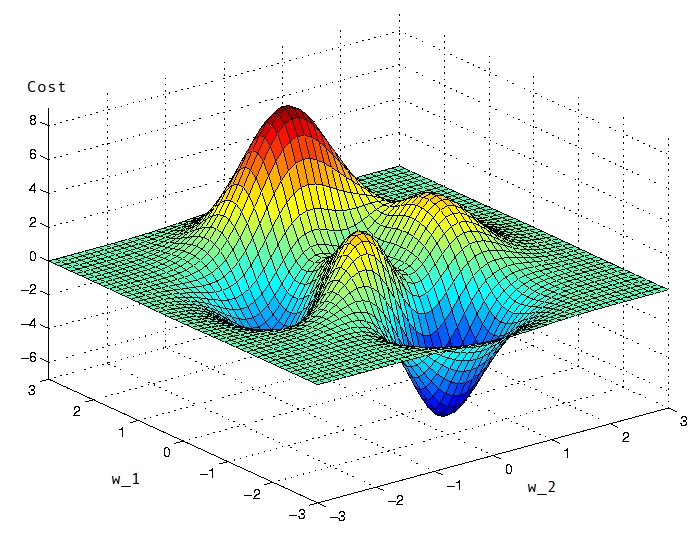
\includegraphics[width=0.5\linewidth]{error_plot}
    \caption{Imagine $z-axis = C(w)$, $y-axis = w_{0}$, and $x-axis = w_{1}$, where $C(w) = w_{0} + x_{1} * w_{1} $.}
    \label{fig:error_surface}
  \end{figure}
\end{document}